\documentclass[oneside,senior,etd]{BYUPhysForDegree}

\usepackage[utf8]{inputenc}
\usepackage{rotating} 

\usepackage[russian]{babel}
\usepackage{amsfonts} % Пакеты для математических символов и теорем
\usepackage{amstext}
\usepackage{amssymb}
\usepackage{amsthm}
\usepackage{graphicx} % Пакеты для вставки графики
\usepackage{subfig}
\usepackage[unicode]{hyperref}
\usepackage[nottoc]{tocbibind} % Для того, чтобы список литературы отображался в оглавлении
\usepackage{verbatim} % Для вставок заранее подготовленного текста в режиме as-is
\usepackage{listings}

\usepackage{commath}
\newcommand\Tau{\mathcal{T}}
\newcommand{\R}{\mathbb{R}}
\usepackage{color}
\usepackage[colorinlistoftodos, prependcaption]{todonotes}
\usepackage{multirow}
\usepackage[T1]{fontenc}
\newcommand*{\MyIndent}{\hspace*{0.2cm}}%

\Chair{Кафедра системного программирования}
\Lab{~}
\Year{2022}
  \Month{Май}
  \City{Москва}
  \AuthorText{Автор}
  \Author{Богатенкова Анастасия Олеговна}
  \AuthorEng{}
  \AcadGroup{628}
  \TitleTop{Распознавание рукописного текста на русском языке}
  %\TitleMiddle{}
  \TitleBottom{} % leave empty if you don't need it
  \TitleTopEng{Handwritten Russian text recognition}
  \TitleBottomEng{} % leave empty if you don't need it  
  %\docname{Курсовая работа}
  %\docname{Выпускная квалификационная работа}
  \docname{Магистерская диссертация}
  \Advisor{Корухова Людмила Сергеевна}
  \AdvisorDegree{к.ф.-м.н.}
  \Consultant{Беляева Оксана Владимировна}
  \ConsultantDegree{}
  
\Abstract{Задача автоматического распознавания рукописного текста является важной состаляющей в процессе анализа электронных документов.
Несмотря на необходимость решения данной задачи на достаточно высоком уровне, ее решение все еще далеко от идеала.
Одной из основных причин сложности распознавания рукописного текста является недостаточное количество данных, используемых для обучения моделей распознавания.
При этом, если для английского языка существуют объемные и разнообразные наборы данных, то для русского языка проблема встает более остро и усугубляется большим разнообразием сложных почерков.
В данной работе рассматривается решение задачи распознавания рукописного текста на русском языке с помощью модели, показывающей наилучшие результаты для английских текстов.
Более того, предлагается способ расширения обучающего набора данных, который можно использовать для генерации рукописных текстов на любом языке.}

\AbstractEng{Automatic handwriting recognition is an important component in the process of electronic documents analysis.
Despite the need to solve this problem at a sufficiently high level, its solution is still far from ideal.
One of the main reasons for the complexity of handwriting recognition is the insufficient amount of data used to train recognition models.
At the same time, in comparison with the English language where data sets are voluminous and diverse, for the Russian language the problem is more acute and is exacerbated by a large variety of complex handwriting.
This work describes the solution of the problem of handwriting recognition in Russian using a model that shows state of the art results for English texts.
Moreover, a method is proposed for extending the training dataset, which can be used to generate handwritten texts in any language.}


%%%% DON'T change this. It is here because .sty does not support cyrillic cp properly %%%%
\University{Московский государственный университет имени М.В. Ломоносова}
\Faculty{Факультет вычислительной математики и кибернетики}
\GrText{гр.}
\AdvisorText{Научный руководитель}
\ConsultantText{Научный консультант}
\AbstractText{Аннотация}

\begin{document}
\fixmargins
\makepreliminarypages

\oneandhalfspace

\tableofcontents

\section{Введение}
\label{sec:Chapter0} \index{Chapter0}


\todo[inline]{В этой части надо описать предметную область, задачу из которой вы будете решать, объяснить её актуальность (почему надо что-то делать сейчас?).
Здесь же стоит ввести определения понятий, которые вам понадобятся в постановке задачи.}


 % Введение
\section{Постановка задачи}
\label{sec:Chapter1} \index{Chapter1}

Задача распознавания рукописного текста (HTR) заключается в разработке моделей и алгоритмов,
способных преобразовывать изображение рукописного текста в цифровой формат (последовательность символов).

Математическая постановка задачи выглядит следующим образом.

\begin{itemize}
    \item[] Пусть $x^{m \times n \times c}$ -- входное изображение шириной $m$ и высотой $n$, $c$ -- число каналов ($c=1$ для черно-белого изображения).
    \item[] Пусть $y^t=(y_1,\dots,y_t),~y_i \in A,~i=1,\dots t$ -- выходная последовательность символов из алфавита $A$.
    \item[] Пусть $X=\{x^{m \times n \times c},~m,n>0,~c\in\{1,3\}\},~Y=\{y^t,~0<t\leqslant T\}$ -- множества входных изображений и выходных последовательностей соответственно.
\end{itemize}

Задача распознавания рукописного текста состоит в определении отображения:
\[ X \rightarrow Y \]
задающего для каждого изображения рукописного текста его цифровое представление в виде последовательности символов.

Согласно главе~\ref{sec:Chapter0} в решении данной задачи хорошо себя зарекомендовали модели глубокого обучения.
Такие модели требуют обучения, соответственно необходим большой по объему и вариативный обучающий набор данных.
Как правило, для расширения набора данных используют аугментацию данных -- случайное преобразование имеющихся данных,
а также генерацию синтетических данных, обладающих достаточной реалистичностью.
При этом, именно создание исскусственных данных может существенно влиять на результат обучения в рамках текущей задачи в силу того,
что оно позволяет генерировать новые сочетания символов/слов и предотвращает переобучение модели на конкретных наборах слов.
Поэтому исследование эффективности методов генерации синтетических данных может помочь улучшить результаты обучаемых моделей.

Как было сказано в главе~\ref{sec:Chapter0}, одним из наиболее распространенных методов расширения обучающего набора данных
является генерация изображений текста на основе рукописных шрифтов.
Тем не менее, в научной литературе не упоминается применение данного метода для распознавания рукописного текста на русском языке.
Соответственно, нет информации и об его реализации.

Таким образом, в силу вышеописанных рассуждений, предлагается выполнить следующее:
\begin{itemize}
    \item Исследовать существующие обучающие наборы данных -- изображений рукописных слов на русском языке, методы их предобработки и аугментации;
    \item Исследовать архитектуры нейросетевых моделей распознавания рукописного текста, выбрать лучшие для дополнительных исследований;
    \item Разработать и реализовать метод генерации дополнительного обучающего набора данных на основе рукописных шрифтов;
    \item Исследовать влияние различных методов генерации дополнительного набора данных на качество предсказания моделей;
    \item Разработать и реализовать метод, позволяющий предсказывать по изображению рукописного слова текст, представленный на изображении;
    \item Провести оценку качества реализованного метода.
\end{itemize}
 % Постановка задачи
\section{Обзор существующих решений}
\label{sec:Chapter2} \index{Chapter2}

% Описание задачи и её типов
Распознавание рукописного текста (HTR) позволяет переводить рукописный текст в цифровой формат.
Основная сложность задачи заключается в значительной вариативности рукописного текста.
Почерк каждого человека отличается от других людей (межличностная изменчивость),
и даже один и тот же человек пишет одно и то же слово по-разному (внутриличностная изменчивость)~\cite{sueiras2021continuous}.
Такие факторы, как скорость письма, размер шрифта, тип используемой бумаги и ручки и даже эмоциональное состояние,
еще больше увеличивают эту изменчивость.

В зависимости от характера исходных данных существуют два основных направления исследования задачи.
С одной стороны, решается задача распознавания рукописного текста на бумажной странице,
отсканированной в цифровое изображение, называемая автономным (офлайн) распознаванием рукописного текста.
С другой стороны, существует так называемое онлайн-распознавание рукописного ввода,
заключающееся в распознавании рукописного текста по непрерывным данным о положениях $(x, y)$ ручки,
полученных при написании этого текста.
Эти данные обычно получают путем ввода непосредственно на сенсорном экране.
Мы ограничимся исследованием задачи офлайн распознавания рукописного текста.

% распознавание рукописного текста в контексте анализа документов в целом
Проблема распознавания рукописного текста в автономном режиме открывает несколько направлений исследований, которые еще далеко не полностью решены.
Для распознавания рукописного текста в документе необходимо, чтобы изначально были определены части изображения, содержащие рукописный текст.
Кроме того, при необходимости текст может быть сегментирован в строки и слова.
Изображение текста может встречаться в таблицах или формах, перекрываться с другими элементами страницы, такими как изображения, схемы или графики.
Текст может быть написан на разных языках с разными наборами символов (т.е. алфавитами), например на китайском, арабском или японском.

Нахождение различных типов элементов (например, рукописный текст, печатный текст, графики и т.д.)
в отсканированных изображениях документов называется \textit{анализом макета} (layout analysis).
Это отдельная сложная и до сих пор нерешённая задача, которая широко исследуется в настоящее время~\cite{binmakhashen2019document}.

% сегментация текста
После нахождения текста на изображении, его распознавание обычно включает в себя несколько шагов~\cite{plamondon2000online}.
В самом общем случае изображение с текстом может содержать параграф, состоящий из нескольких строк.
В этом случае чаще всего текст разбивается на строки.
Однако сегментация строк не является тривиальной из-за наклона строк, наклона символов внутри строки и того факта,
что некоторые символы в соседних строках могут перекрываться другими.
Модели распознавания могут быть применены непосредственно к текстовым строкам, либо их можно разбить на слова, и распознавание выполнять на уровне слов.
Большинство современных алгоритмов HTR можно применять либо к строкам, либо к словам, которые являются частным случаем коротких строк.

% наборы данных и аугментация
Для обучения моделей распознавания рукописного текста с использованием методов глубокого обучения
требуются наборы данных изображений рукописного текста, должным образом аннотированные текстом, присутствующим в каждом изображении.
Существует несколько общедоступных наборов данных, некоторые из них содержат изображения отдельных символов,
другие содержат изображения слов, строк и абзацев.
В любом случае объем аннотированных данных, доступных для обучения моделей, ограничен и требует рассмотрения возможности
использования стратегий увеличения данных (аугментации) для обучения моделей.

В следующих секциях описано, каким образом измеряется качество работы методов распознавания рукописного текста.
Кроме того, описаны наборы данных с рукописным текстом на русском языке, а также методы предобработки и аугментации данных.
В заключение, перечисляются основные архитектуры нейросетевых моделей, применяемых для решения задачи распознавания рукописного текста.
Модели в основном разрабатываются для текстов на английском языке, тем не менее существуют решения для русского языка,
которые также описаны в контексте других моделей.


\subsection{Метрики оценки качества}
\label{subsec:evaluation-metrics}

Двумя основными метриками, обычно используемыми для оценки моделей распознавания рукописного текста на уровне слов и строк,
являются \textit{частота ошибок символов} (Character Error Rate, CER) и \textit{частота ошибок слов} (Word Error Rate, WER).

CER измеряет расстояние Левенштейна~\cite{levenshtein1966binary} между предсказанной и реальной последовательностью символов слова.
Расстояние Левенштейна, также иногда называемое расстоянием редактирования,
представляет собой метрику для измерения разницы между двумя последовательностями.
Неформально расстояние Левенштейна между двумя словами (предсказание модели и реальное слово) --
это минимальное количество вставок, удалений или замен, необходимых для преобразования предсказания в правильное слово,
делённое на длину правильного слова, как показано в уравнении~(\ref{eq:cer}).

\begin{equation}
    \label{eq:cer}
    CER(prediction,real)=\frac{substitutions+insertions+deletes}{len(real)}
\end{equation}

Частота ошибок в словах (WER) определяется аналогично CER путем вычисления минимального количества вставок, замен и удалений слов,
необходимых для перехода от текстовой строки, предсказанной моделью, к реальной текстовой строке.

В некоторых работах наравне с частотой ошибок символов и частотой ошибок слов используется \textit{точность} (accuracy).
Данная метрика используется для любых текстовых строк, содержащих как слова, так и предложения.
Точность описывается формулой~(\ref{eq:accuracy}), в которой под равенством подразумевается полное совпадение двух строк.
Данная метрика позволяет оценить качество модели более грубо, так как ошибка в одном символе сильно понижает результирующее значение.

\begin{equation}
    \label{eq:accuracy}
    accuracy(prediction,real)=\frac{\sum_{i=1}^N pred_i = real_i}{N}
\end{equation}


\subsection{Наборы данных}
\label{subsec:datasets}

Существует не так много общедоступных наборов данных на русском языке для обучения моделей и сравнения результатов.
На текущий момент известно два набора данных со словами на кириллице:
\begin{itemize}
    \item Cyrillic Handwriting Dataset\footnote{\url{https://www.kaggle.com/datasets/constantinwerner/cyrillic-handwriting-dataset}};
    \item HKR\footnote{\url{https://github.com/abdoelsayed2016/HKR_Dataset}}.
\end{itemize}

Кроме того, найдено два набора данных русских символов, являющиеся не очень популярными:
\begin{itemize}
    \item CoMNIST\footnote{\url{https://github.com/GregVial/CoMNIST}};
    \item База сегментированных рукописных символов\footnote{\url{https://drive.google.com/folderview?id=0B0EQUc5HmgcGS0l2RDlKenlpNnc&usp=sharing}}.
\end{itemize}

Основная информация о наборах данных представлена в таблице~\ref{tab:datasets}.

\begin{table}[h!]
    \centering
    \begin{tabular}{|p{4cm}|p{7cm}|p{3cm}|}
        \hline
        \textbf{Название} & \textbf{Описание} & \textbf{Размер} \\
        \hline
        \hline
        Cyrillic Handwriting Dataset & Набор русских текстов длиной $\leqslant$ 40 символов, собранный из различных интернет-ресурсов & train=72286 test=1544 \\
        \hline
        HKR~\cite{nurseitov2021handwritten} & Набор из русских (95\%) и казахских (5\%) слов и предложений: ключевые слова, поэмы и алфавит & train=45470 val=9359 test1=5057 test2=5057 \\
        \hline
        CoMNIST & Символы -- русские заглавные буквы, собран при помощи краудсорсинга & более 28000 \\
        \hline
        База сегментированных рукописных символов & Обширная база из строчных и прописных рукописных символов, а также цифр & всего 120750 символов \\
        \hline
    \end{tabular}
    \caption{Наборы данных с кириллицей}
    \label{tab:datasets}
\end{table}

\paragraph{Cyrillic Handwriting Dataset.}{Данный набор данных был опубликован в 2022 году, поэтому еще нет работ, содержащих результаты его обработки.
Этот набор очень интересен с точки зрения разнообразия данных: в него входят студенческие конспекты, заполненные формы, электронные рукописные документы.
Изображения содержат раличного рода шумы и неоднородный фон, в некоторых случаях на изображение одного слова попадают части другого или разлиновка листа.
Набор содержит как слова, так и предложения, некоторые метки могут содержаться несколько раз (например, слово <<что>>), но есть и уникальные.
Согласно табице~\ref{tab:datasets} набор данных состоит из более 70 тысяч обучающих примеров, что также является его существенным достоинством.
Кроме того, он является открытым как для научных исследований, так и для коммерческого использования.
Примеры изображений, встречающиеся в наборе данных, представлены на рисунке~\ref{fig:cyrillic-examples}}

\begin{figure}[h!]
    \centering
    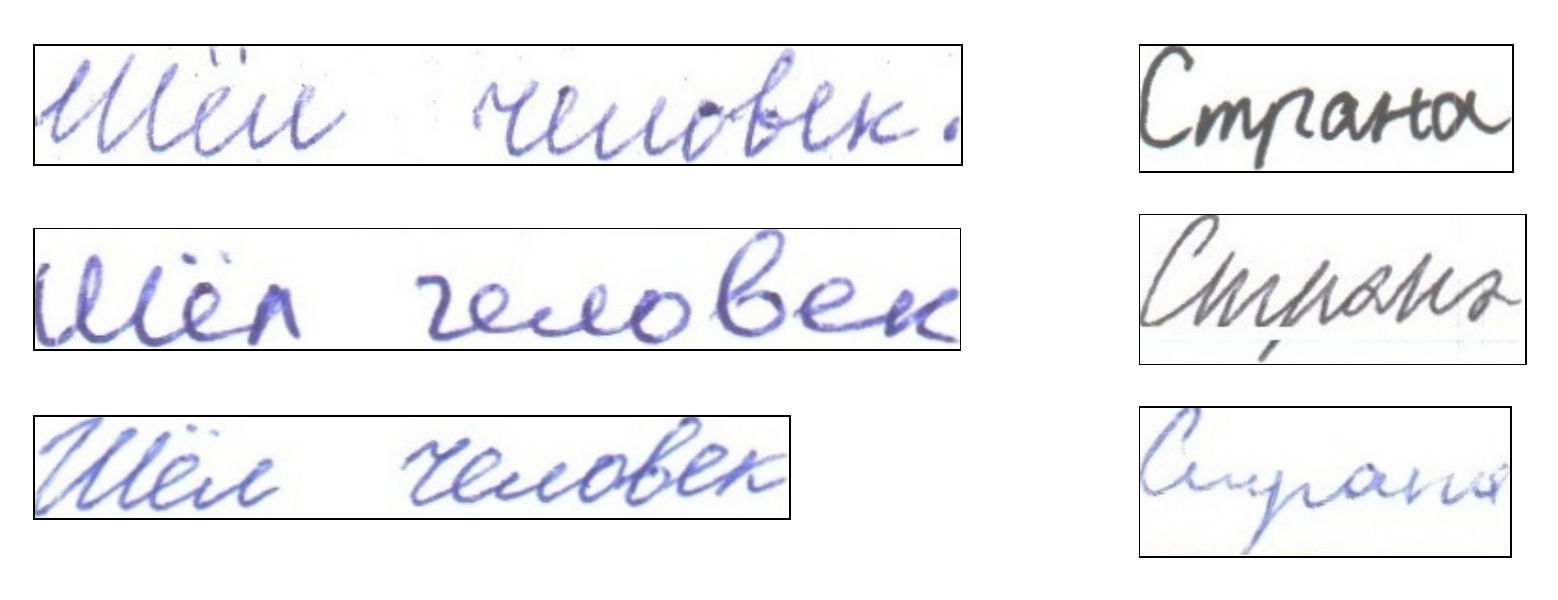
\includegraphics[width=\textwidth]{img/cyrillic}
    \caption{Примеры изображений набора Cyrillic Handwriting Dataset}
    \label{fig:cyrillic-examples}
\end{figure}

\paragraph{HKR.}{Наиболее популярным набором данных, упоминаемым в научной литературе, является набор казахских и русских слов и предложений~\cite{nurseitov2021handwritten}.
Всего в нем содержится более 60 тысяч изображений слов и предложений, написанных примерно 200 различными почерками.
Он создавался путем заполнения однотипных форм, поэтому имеет одну особенность -- в нем содержится большое количество копий одного и того же текста, написанного разными почерками.
Отдельно авторами дается разбиение набора данных\footnote{\url{https://github.com/bosskairat/Dataset}} на тренировочный, валидационный и два тестовых набора.
Первый тестовый набор содержит слова, которых нет в тренировочном наборе, но написанные почерками, присутствующими в тренировочном наборе.
Напротив, второй тестовый набор содержит слова, которые есть в тренировочном наборе, но написанные <<новыми>> почерками.
Эта особенность позволяет провести анализ того, на что в большей степени обращает внимание обучаемая модель: новые способы написания символов или новые сочетания.
Несмотря на значительный объем набора, изображения в нем достаточно хорошего качества и относительно однообразны.
Таким образом, произвольное изображение рукописного текста из <<реального мира>> совершенно не похоже на то, что содержится в описанном наборе данных.
В добавление к этому, использование данного набора ограничивается научными исследованиями, для его использования в коммерческих целях необходимо обратиться к его авторам.
Примеры изображений, встречающиеся в наборе данных, представлены на рисунке~\ref{fig:hkr-examples}}

\begin{figure}[h!]
    \centering
    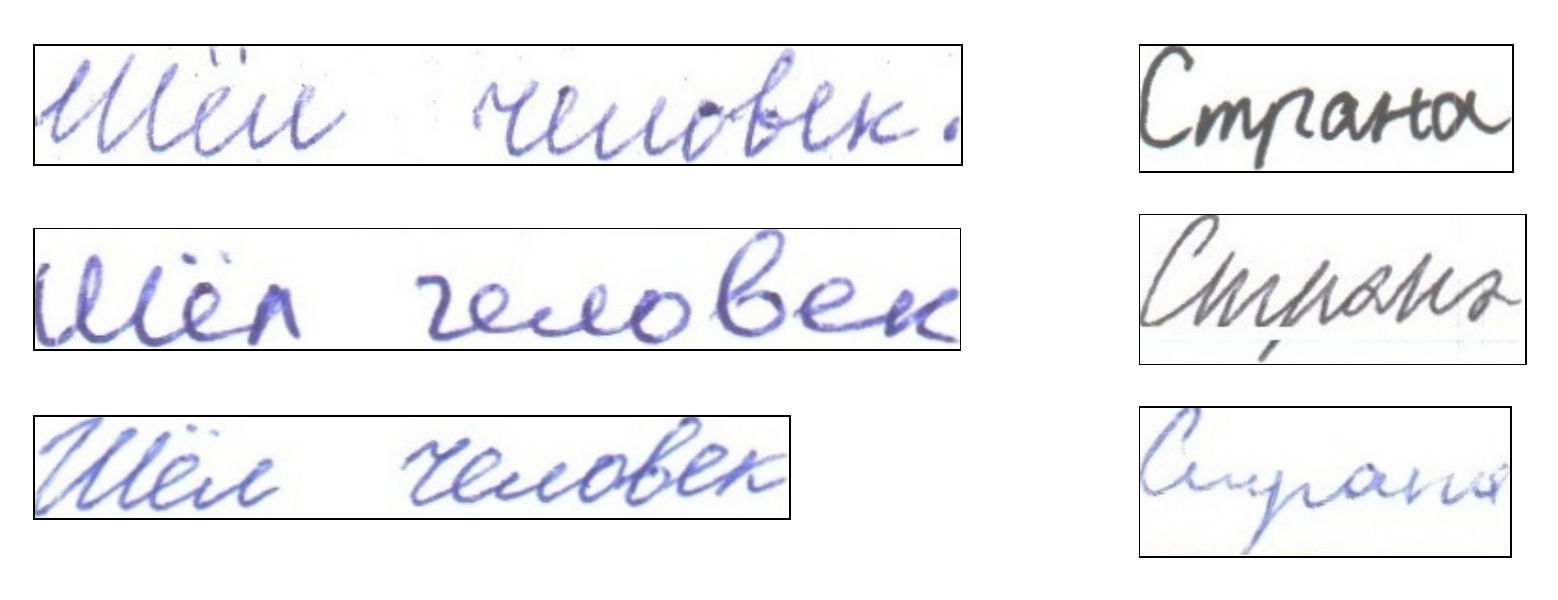
\includegraphics[width=\textwidth]{img/hkr}
    \caption{Примеры изображений набора HKR}
    \label{fig:hkr-examples}
\end{figure}

\paragraph{Символьные наборы данных.}{Наборы рукописных символов могут пригодиться при распознавании рукописных текстов, если используется обучение модели классификации символов.
Достаточно известным набором является собранный добровольцами CoMNIST, который имеет несколько недостатков.
Он содержит только заглавные символы, соответственно область его применения резко сужается.
Более того, при разметке символы пишутся людьми на экране телефона, планшета или ноутбука, что сильно отличается от написанных текстов на бумаге.
Набор создавался методом краудсорсинга, поэтому добавляется проблема корректности собранных данных.

Существует также малоизвестная база сегментированных символов, в которой содержатся все заглавные и строчные символы русского алфавита.
Каждый из символов написан более 1500 различными почерками, также присутствует более 300 экземпляров каждой цифры.
Изображения создавались путем заполнения форм от руки с последующей бинаризацией изображения, поэтому выглядят они менее искусственно.
Несмотря на непопулярность в литературе, у данной базы есть большой потенциал для дальнейших исследований.}


\subsection{Методы предобработки данных}
\label{subsec:preprocessing}

Несмотря на явное различие в написании текста на кириллице и латинице, в рукописных текстах есть некоторое сходство,
которое позволяет применять похожие методы предобработки данных к текстам на разных языках.
В кириллических рукописных текстах аналогично латинским присутствует наклон символов,
текст пишется слева направо -- соответственно может встречаться наклон строк.
Кроме того, в строках могут встречаться символы, выходящие за пределы основной строки --
например, заглавные символы или символы с верхними или нижними петлями.
Текст, как правило, пишется на бумаге, которая может иметь дефекты, некоторые недостатки может иметь и сам рукописный текст.
Поэтому имеет смысл рассматривать методы предобработки данных, используемые для текстов на латинице (в частности, для английского языка).
Далее будут более подробно описаны некоторые методики, позволяющие улучшить качество входных данных и привести их к более нормализованному виду.

\subsubsection{Удаление шума и бинаризация}
\label{subsubsec:binarization}

Оцифрованное изображение рукописного текста подвержено множеству источников шума, поэтому даже человеку иногда сложно его распознать.
Бумага может содержать следы, может быть не совсем белой или испорченной.
Если лист бумаги тонкий, может быть виден также текст, написанный обратной стороне (эффект просвечивания).
В процессе оцифровки на изображении могут появиться артефакты, вызванные, загрязнениями сканера.
Шумоподавление изображения -- это первый шаг в обработке и стандартизации изображения.
Его цель состоит в том, чтобы получить изображение в градациях серого, в котором текст имеет четкие черные штрихи,
а фон не содержит элементов, влияющих на предсказания модели.

Крайний случай устранения шумов на изображении -- бинаризация.
В результате бинаризации изображение становится чёрно-белым, без градаций серого.
Пример предполагаемых результатов работы бинаризации представлен на рисунке~\ref{fig:binarization}.
\begin{figure}[h!]
    \centering
    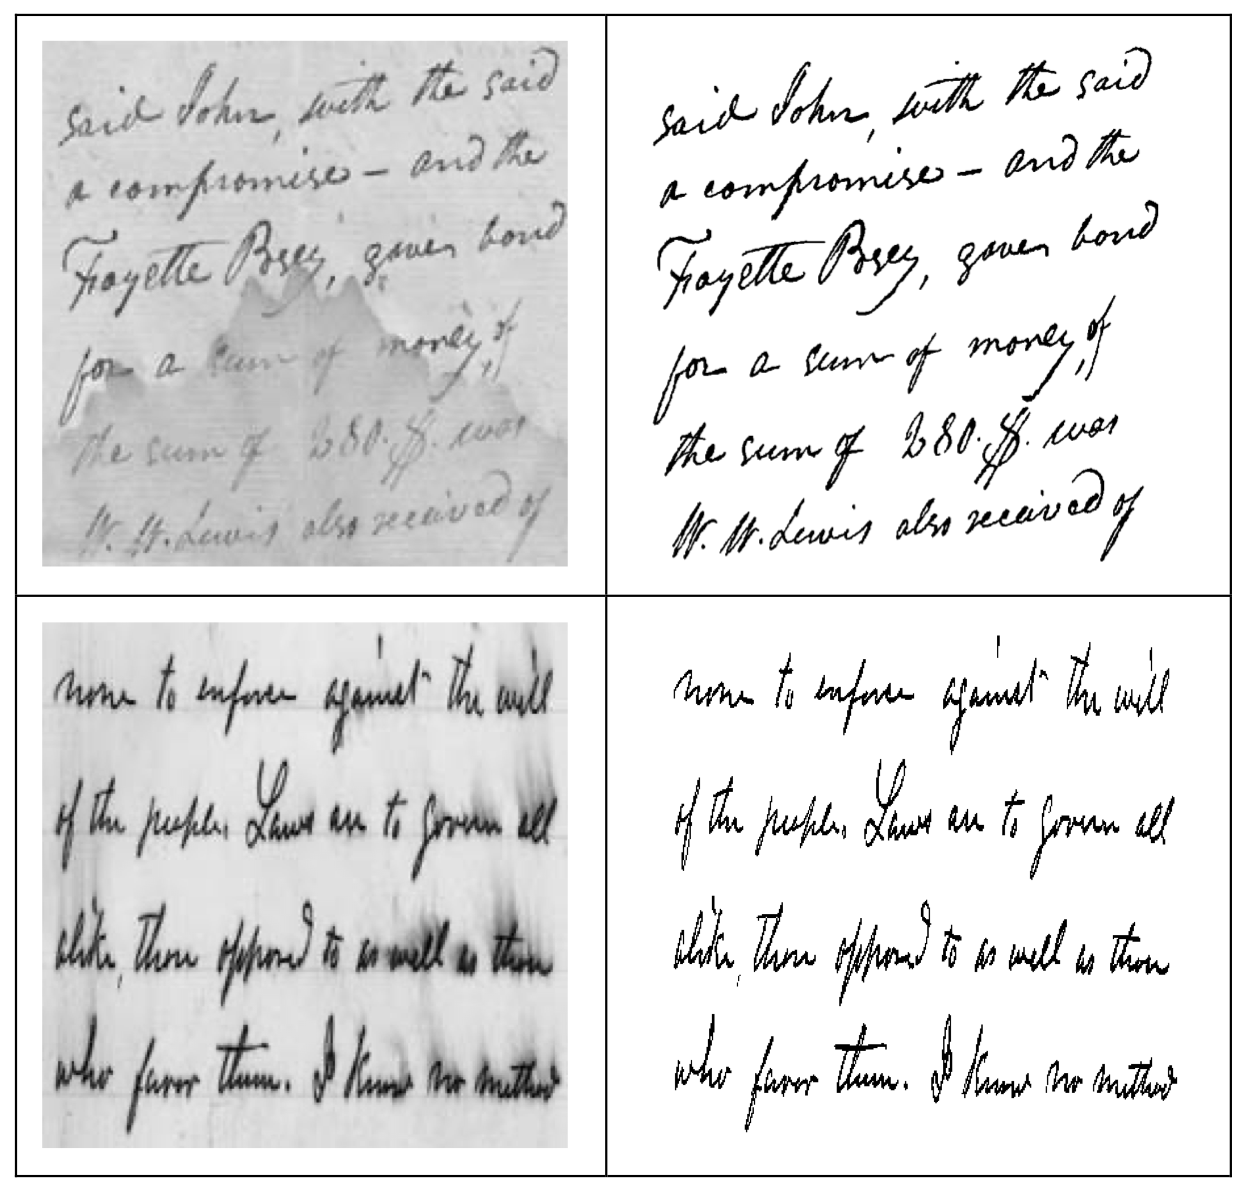
\includegraphics[width=0.6\textwidth]{img/binarization}
    \caption{Пример документов до (слева) и после (справа) бинаризации}
    \label{fig:binarization}
\end{figure}

Существует большое количество работ, посвящённых решению задачи бинаризации документов, а также обзоров методов~\cite{mustafa2018binarization}.
В частности, один из самых простых и эффективных методов -- использование адаптивного порога бинаризации, вычисляющегося для небольших участков изображения.


\subsubsection{Исправление наклона строки и символов}
\label{subsubsec:slope-slant-correction}

\textit{Наклон строки} -- это наклон текстовой строки документа относительно горизонтальной линии.
Как правило, он появляется, когда текст пишется на пустой странице без предварительной разлиновки.
На верхнем изображении рисунка~\ref{fig:slope-slant} показан пример наклона строки с положительным углом.
Коррекция наклона может выполняться на уровне страницы, а также на уровне строки или даже на уровне слова.

\textit{Наклон символов} -- распространённое свойство, используемое в процессе обучения письму.
Именно поэтому он очень популярен и является одним из основных источников вариативности рукописного текста,
что затрудняет его распознавание с помощью автоматических систем.
Идентификация и исправление наклона являются критически важными аспектами распознавания рукописного текста,
поскольку многие алгоритмы распознавания, использующие изображения рукописного текста в качестве входных данных,
обычно используют подход, который анализирует изображение столбец за столбцом.
К таким моделям можно отнести полносвязные нейронные сети (многослойный перцептрон, рекуррентные нейронные сети),
у моделей, использующих свёрточные сети, такой проблемы нет~\cite{sueiras2021continuous}.

В любом случае коррекция наклона символов обеспечивает снижение вариативности рукописного текста,
что облегчает его распознавание вне зависимости от типа используемой модели.
Поэтому исправление наклона символов, наряду с шумоподавлением, является самым распространенным методом предварительной обработки при решении задачи распознавания рукописного текста.
Коррекция наклона символов обычно выполняется в два этапа: определение угла наклона строк, а затем применение преобразования для коррекции этого угла.
Зачастую, исправление наклона символов иногда частично выполняется одновременно с исправлением наклона строк,
поскольку исправление угла наклона строки изменяет угол наклона символов на ту же величину.
Пример исправления наклона строки с последующим исправлением наклона символов показан на рисунке~\ref{fig:slope-slant}.

\begin{figure}[h!]
    \centering
    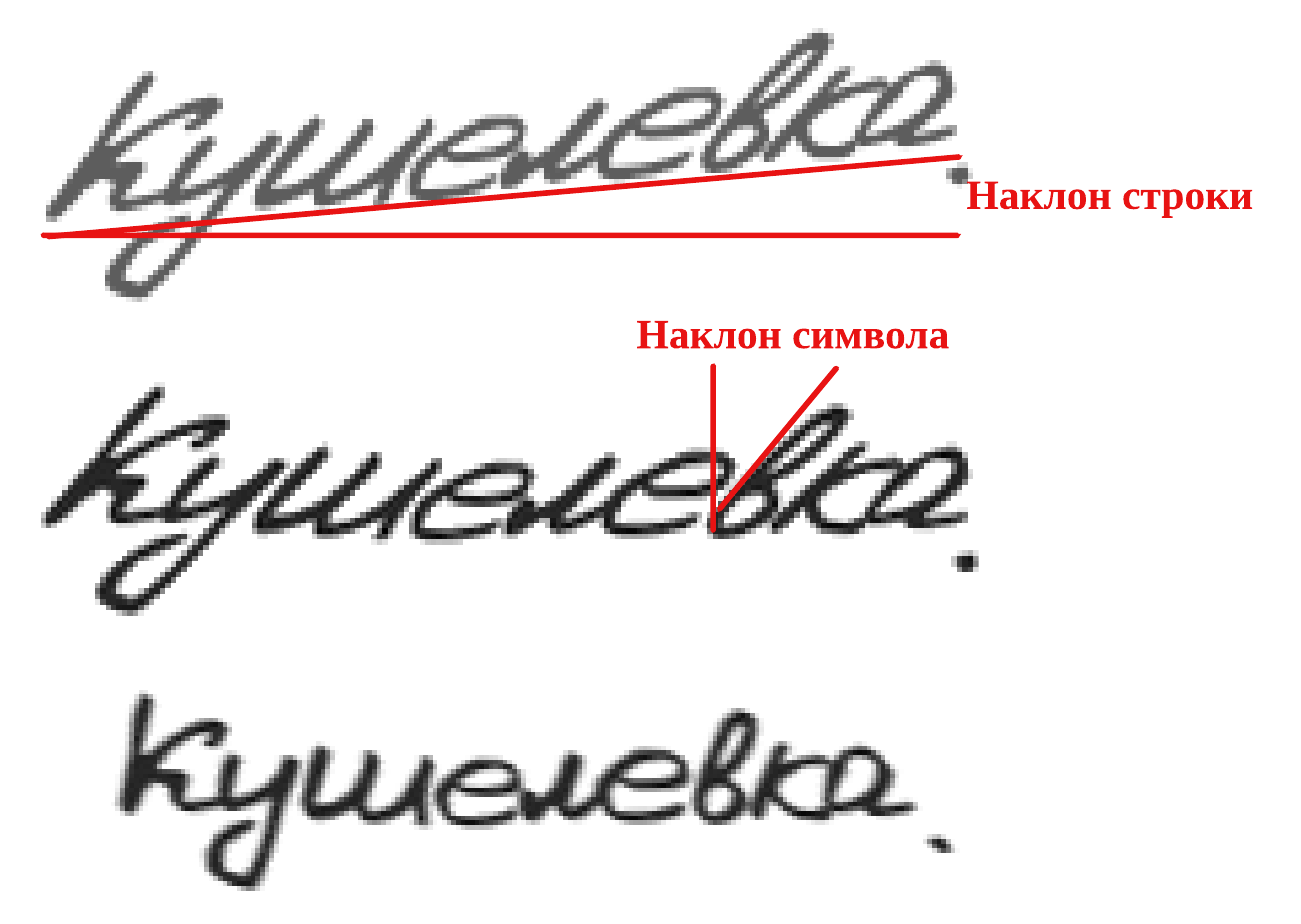
\includegraphics[width=0.5\textwidth]{img/slant-slope}
    \caption{Пример исправления наклона строки и символов (внизу исправленный вариант)}
    \label{fig:slope-slant}
\end{figure}

Одним из самых популярных методов коррекции наклона строки является преобразование Хафа~\cite{duda1972use} из-за его надёжности и простоты.
Однако этот метод является вычислительно сложным.
Поэтому несколько авторов предложили варианты, которые уменьшают размер пространства Хафа~\cite{pal1996improved,boukharouba2017new}, хотя вычислительные затраты остаются высокими.

В качестве альтернативы другие авторы определяют угол наклона строки, оценивая линию, которая лучше всего соответствует набору пикселей на изображении.
Например, в работе~\cite{gupta2014efficient} используется линейная регрессия координат x, y пикселей в основной области текста.

Другой широко используемый метод, как для определения наклона строки, так и для определения наклона символов, основан на профилях проекций, например~\cite{kavallieratou2002skew} и~\cite{pastor2004projection}.
Горизонтальная проекция текстовых пикселей используется для определения угла наклона строки, а вертикальная проекция используется для определения угла наклона символов.
Подобные методы довольно чувствительны к присутствию шума на изображении, и для их применения необходимо сначала использовать методы, упомянутые в разделе~\ref{subsubsec:binarization}.

Помимо метода, использующего профили проекций, существуют и другие методы исправления угла наклона символов.
В работе~\cite{gupta2012novel} предложен алгоритм определения угла наклона, который основан на способности фильтра Габора обнаруживать направленные текстуры.
В той же работе описан второй метод оценки угла наклона, который использует преобразование Фурье для преобразования изображения слова в спектр Фурье.
Повторение точек вдоль заданного направления активирует частотное пространство в его перпендикулярном направлении, и это направление соответствует углу наклона.
Другой пример можно в работе~\cite{vinciarelli2001new}, где метод определения угла наклона символов основан на гипотезе о том,
что изображение слова наклоняется, когда количество столбцов, содержащих непрерывные штрихи, максимально.


\subsection{Расширение обучающих наборов данных}
\label{subsec:augmentation-generation}

Одной из важнейших проблем при решении любых задач с использованием машинного обучения является недостаточный объем обучающих данных.
Аугментация -- техника, применяемая в процессе обучения моделей и позволяющая снизить серьезность данной проблемы.
Аугментация данных позволяет с помощью некоторых преобразований из существующих данных получить новые, несколько отличающиеся от исходных.
Использование этой техники в процессе обучения позволяет получать бесконечное количество каким-то образом различающихся обучающих примеров.
Тем самым аугментация позволяет получить модели, более устойчивые к изменениям входных данных и показывающие более высокое качество решения задачи.

Несмотря на безусловные плюсы использования аугментации при обучении моделей машинного обучения, этот метод не является панацеей и не позволяет полностью избавиться от проблем.
Любое автоматическое преобразование данных, каким бы случайным и естественным оно ни было, не сможет в полной мере заменить новые реальные данные.
Тем не менее, аугментация широко используется с поправкой на то, что многого от нее ожидать не следует.
Распознавание рукописного текста -- не исключение, практически в любой работе используются как минимум простейшие случайные изменения обучающих данных.

Помимо аугментации, для решения некоторых задач существует возможность использовать данные, сгенерированные автоматически -- синтетические данные.
В некоторых случаях можно обойтись только синтетическими примерами, однако в подавляющем большинстве случаев сгенерированные данные
являются лишь частью обучающего корпуса и должны быть максимально разнообразными, чтобы не спровоцировать переобучение модели.
Этот способ также приемлем для расширения набора данных из рукописных слов/предложений, однако его нельзя использовать без добавления реальных данных.

\subsubsection{Аугментация данных}
\label{subsubsec:augmentation}

Как правило, при обучении моделей распознавания рукописного текста применяются достаточно распространённые случайные изменения:
изменение размера изображения, искажение перспективы, размытие и повышение резкости, добавление случайных шумов, растяжение и сжатие изображения,
случайные повороты, эрозия и дилатация, афинные преобразования и упругие деформации~\cite{sueiras2021continuous}.

\begin{figure}[h!]
    \centering
    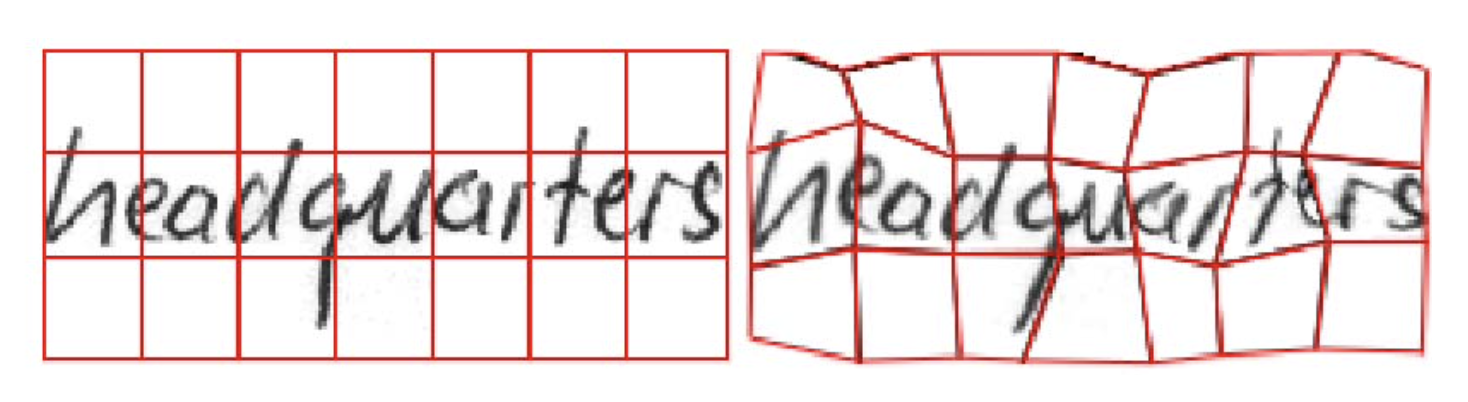
\includegraphics[width=0.4\textwidth]{img/aug_local}
    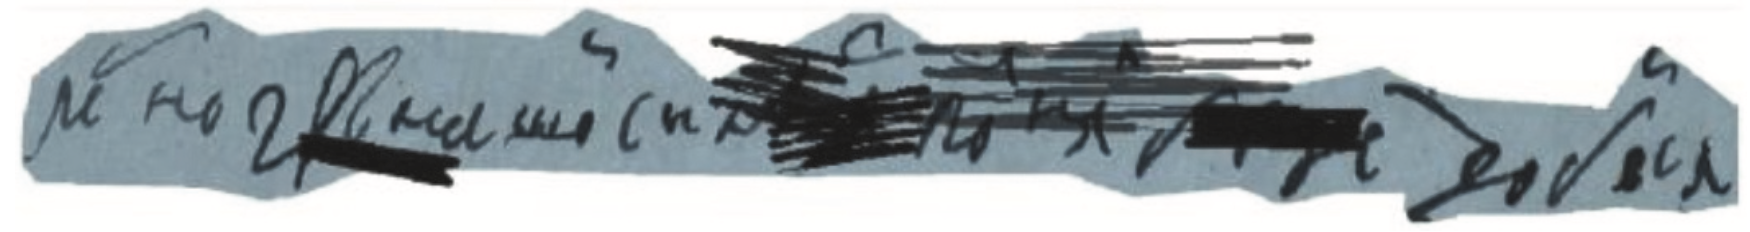
\includegraphics[width=0.5\textwidth]{img/aug_blots}
    \caption{Примеры аугментации с помощью локальных искажений (слева) и сгенерированных <<рукописных>> пятен (справа)}
    \label{fig:augmentation}
\end{figure}

Еще один способ аугментации описан в работе~\cite{wigington2017data}, где используются локальные искажения на основе сетки контрольных точек изображения (см. рисунок~\ref{fig:augmentation}).
Этот метод отличается от простых афинных преобразований тем, что работает по-разному с маленькими частями изображения, а не искажает его целиком.

Помимо случайных шумов, которые не добавляют реализма изображению, используются и другие методы вставки дополнительных <<объектов>>.
В статье~\cite{shonenkov2021stackmix} описывается аугментация методом рисования на изображении пятен, похожих на рукописные зачеркивания (см. рисунок~\ref{fig:augmentation}).
Для этого на изображении выбираются случайные области, где фиксируются произвольные точки, с помощью которых проводятся кривые Безье.

В некоторых работах аугментация выполняется с помощью дополнительных нейронных сетей, которые обучаются вместе с остальными компонентами модели.
Например, в работе~\cite{krishnan2018word} перед остальными слоями используется сеть пространственного преобразования (STN),
позволяющая менять входные данные путем выбора наиболее релевантных областей изображения и преобразования размера, угла поворота и т. п.~\cite{jaderberg2015spatial}.
В другой работе~\cite{luo2020learn} легковесная нейронная сеть используется для поиска наиболее подходящего набора
контрольных точек, над которым затем производится деформация перемещения наименьших квадратов~\cite{schaefer2006image}.

Несмотря на большое количество разнообразных методов, позволяющих исказить изображение и тем самым позволить обученной
модели стать более устойчивой, они всё же не могут предоставить совершенно новые данные.
В реальности, изображения рукописного текста различаются не только искривлениями букв и пятнами, важную роль играют
сочетания разных символов (то есть сам написанный текст) и то, как соединяются символы в слове (особенности почерка).
Существующие методы аугментации не способны изменить ни то, ни другое.

\subsubsection{Генерация данных}
\label{subsubsec:generation}

Вследствие того, что использование методов аугментации, описанных в секции~\ref{subsubsec:augmentation}, недостаточно для
получения необходимого количества разнообразных обучающих примеров, используется также и другой подход.
Он связан с генерацией новых слов и стилей написания в рукописных текстах.
Такой метод вряд ли позволит получить по-настоящему реалистичные и совершенно новые изображения, однако он может дать
существенный прирост в качестве результатов обучаемых моделей.

Один из интересных способов генерации новых слов и предложений в стиле уже имеющихся слов в наборе данных,
предложили авторы статьи~\cite{shonenkov2021stackmix}, которые также предложили вышеописанный способ рисовать пятна с помощью кривых Безье.
Свой метод они назвали StackMix и состоит он в разбиении слов на символы или подслова, а затем составлении из этих кусочков новых слов (см. рисунок~\ref{fig:generation}).
Такой метод не решает проблему соединения символов и создания новых стилей, зато он может помочь в создании рукописных слов,
которых нет в обучающем наборе данных.

Следующий метод~\cite{krishnan2016generating} состоит в генерации изображений рукописного текста с использованием типографских шрифтов.
Авторы отобрали 90 тысяч уникальных английских слов и сгенерировали 90 миллионов изображений слов с помощью 750 рукописных шрифтов.
Подобный набор слов можно использовать для предобучения моделей распознавания рукописного текста,
однако в силу его однообразности потребуется дообучение на реальных данных, чтобы предотвратить переобучение сети.
Пример генерации изображения рукописного текста с помощью шрифтов приведен на рисунке~\ref{fig:generation}.

В настоящее время является широкоисследуемым целый класс методов генерации рукописного текста,
основанных на использовании генеративно-состязательных сетей (GAN)~\cite{goodfellow2020generative}.
Такие модели в своей основе содержат две нейронных сети: одна из них генерирует примеры (генеративная модель),
а другая пытается отличить подлинные образцы от сгенерированных первой сетью (дискриминативная модель).
Наиболее свежими примерами генеративно-состязательных сетей в области генерации изображений рукописного текста являются
ScrabbleGAN~\cite{fogel2020scrabblegan}, GANwriting~\cite{kang2020ganwriting} и TextStyleBrush~\cite{krishnan2023textstylebrush}.
Пример результата работы ScrabbleGAN приведен на рисунке~\ref{fig:generation}.

\begin{figure}[h!]
    \centering
    \textbf{Stackmix}\par\medskip
    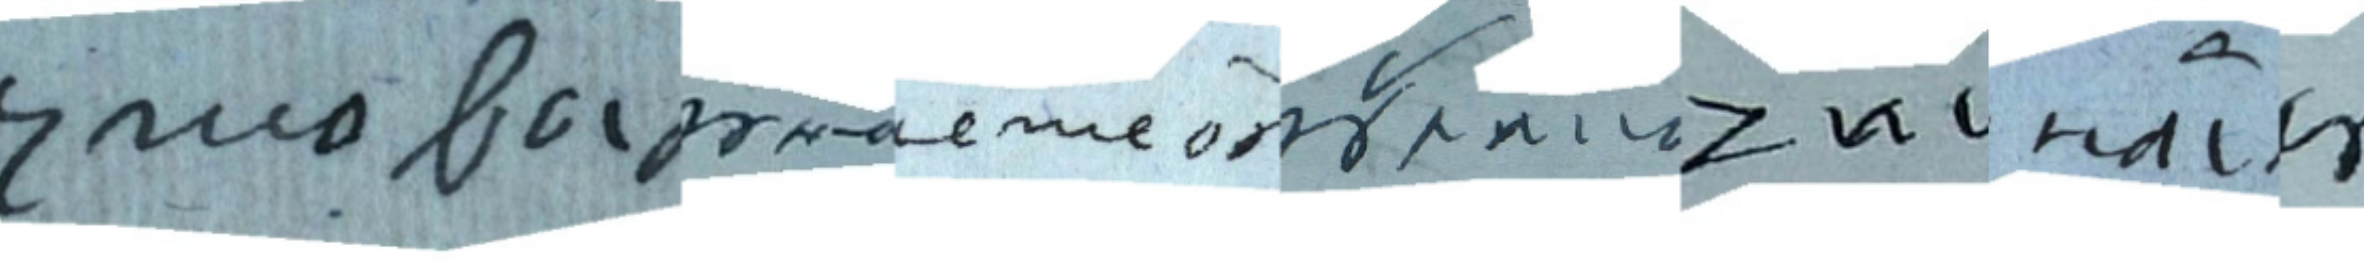
\includegraphics[width=0.9\textwidth]{img/aug_stackmix}
    \textbf{Типографский шрифт}\par\medskip
    \frame{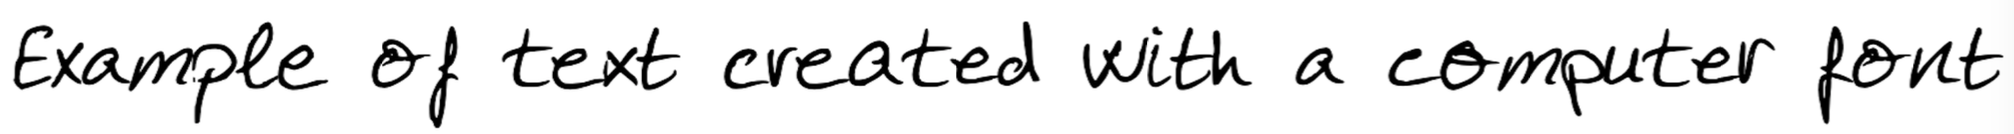
\includegraphics[width=0.9\textwidth]{img/aug_fonts}}
    \textbf{Генеративно-состязательная сеть}\par\medskip
    \frame{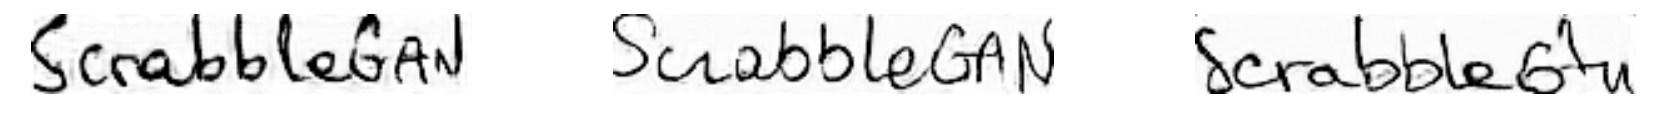
\includegraphics[width=0.9\textwidth]{img/aug_gan}}
    \caption{Примеры сгенерированных изображений}
    \label{fig:generation}
\end{figure}

\textit{ScrabbleGAN}~\cite{fogel2020scrabblegan} -- сеть, состоящая из генератора, дискриминатора и распознавателя символов (OCR).
В данной архитектуре дискриминатор влияет на качество изображения, а распознаватель на читаемость текста на изображении.
Для обучения сеть использует картинки с текстом и сам текст, стили написания текста меняются с помощью вектора шума,
на который домножается входной вектор закодированного текста.
\textit{GANwriting}~\cite{kang2020ganwriting} обладает более сложной архитектурой, в которой присутствуют генераторы текста и стиля,
соответственно используются дискриминатор, классификатор стиля и распознаватель текста.
Вместо одной картинки с текстом, на вход подается группа картинок с текстом, которая формирует конкретный стиль.
Поэтому сеть позволяет сгенерировать текст в разных стилях, которые можно смешивать друг с другом.
\textit{TextStyleBrush}~\cite{krishnan2023textstylebrush} -- наиболее свежая модель, состоящая из 7 нейронных сетей и принимающая на вход картинку со стилем и текст.
Тут также есть генераторы текста и стиля, дискриминатор, классификатор стиля и OCR-модель.
Дополняется этот набор сетью, преобразующей выход генератора стиля в набор векторов, а также генератором стилизованного текста,
который использует и объединяет результаты работы предыдущих генераторов.
Данная модель очень сложна по своей структуре и способна генерировать изображения только тех стилей, на которых была обучена.

Вышеописанные нейросетевые модели генерации обучались и тестировались для английского языка, соответственно помимо недостатка,
связанного с искуссвенностью получающихся изображений, есть и другой -- трудоемкость задачи переобучения сети для другого языка.
Более того, далеко не все авторы делятся исходным кодом описанных ими моделей.

\subsection{Типы нейросетевых моделей}
\label{subsec:networks-description}

Существует большое количество вариаций архитектур моделей, которые используются в исследованиях для решения задачи распознавания рукописного текста.
Если исключить из рассмотрения некоторые детали, модели можно объединить в следующие группы:
\begin{itemize}
    \item Модель для извлечения признаков с последующим применением скрытой марковской модели (HMM).
    \item Свёрточные нейронные сети (CNN).
    \item Рекуррентные нейронные сети (RNN).
    \item Комбинация свёрточной и рекуррентной сетей с CTC на выходе (CNN-RNN-CTC).
    \item Sequence-to-sequence модели (seq2seq).
    \item Трансформеры.
\end{itemize}

 % Обзор существующих решений
\section{Исследование и построение решения задачи}
\label{sec:Chapter3} \index{Chapter3}
\todo[inline]{Здесь надо декомпозировать большую задачу из постановки на подзадачи и продолжать этот процесс, пока подзадачи не станут достаточно простыми, чтобы их можно было бы решить напрямую (например, поставив какой-то эксперимент или доказав теорему) или найти готовое решение.} % Исследование и построение решения задачи
\section{Описание практической части}
\label{sec:Chapter4} \index{Chapter4}

Так как тема данной работы связана с активным использованием техник глубокого обучения, реализация всех методов и экспериментов
сделана на языке программирования \textit{Python}, который предоставляет все необходимые библиотеки, а именно:
\begin{itemize}
    \item \textit{Pillow}, \textit{opencv-python} -- для работы с изображениями, в т.ч. отрисовки шрифтов на изображении;
    \item \textit{albumentations}, \textit{augmixations} -- содержат реализацию основных методов аугментации изображений;
    \item \textit{pandas} -- для удобной работы с табличными данными, в частности для работы с информацией о размеченных наборах данных;
    \item \textit{scikit-learn}, \textit{scikit-image}, \textit{torch}, \textit{torchvision}, \textit{transformers} -- библиотеки с реализацией алгоритмов машинного обучения, а также основных метрик качества;
    \item \textit{datasets} -- для удобной загрузки наборов данных с \textit{huggingface.co}.
\end{itemize}

В рамках выполнения поставленной задачи было создано два публичных репозитория на платформе \textit{github.com}:
\begin{itemize}
    \item \textit{HandwritingGeneration}\footnote{\url{https://github.com/NastyBoget/HandwritingGeneration}}, содержащий код метода генерации синтетических изображений рукописного текста на основе шрифтов;
    \item \textit{hrtr}\footnote{\url{https://github.com/NastyBoget/hrtr)}}, содержащий код загрузки и обработки наборов данных, а также запуска необходимых экспериментов.
\end{itemize}

Помимо этого, для хранения и удобной загрузки созданных синтетических наборов данных использовалась платформа \textit{huggingface.co},
предоставляющая возможность бесплатно загружать и хранить файлы больших размеров.

В следующих секциях дано описание деталей реализации генерации изображений текста на основе рукописных шрифтов,
создания и публикации сгенерированных синтетических наборов данных, а также запуска экспериментов.


\subsection{Реализация генератора изображений рукописного текста}
\label{subsec:handwriting-generation}

В секции~\ref{subsec:synthetic} описан метод полу-автоматической генерации рукописных шрифтов, а также создания синтетических изображений на основе шрифтов.
Для этого был реализован набор модулей с классами-генераторами, доступный по ссылке \url{https://github.com/NastyBoget/HandwritingGeneration}.
На рисунке~\ref{fig:diagram_handwriting_generation} представлена диаграмма реализованных классов.

\begin{figure}[h!]
    \centering
    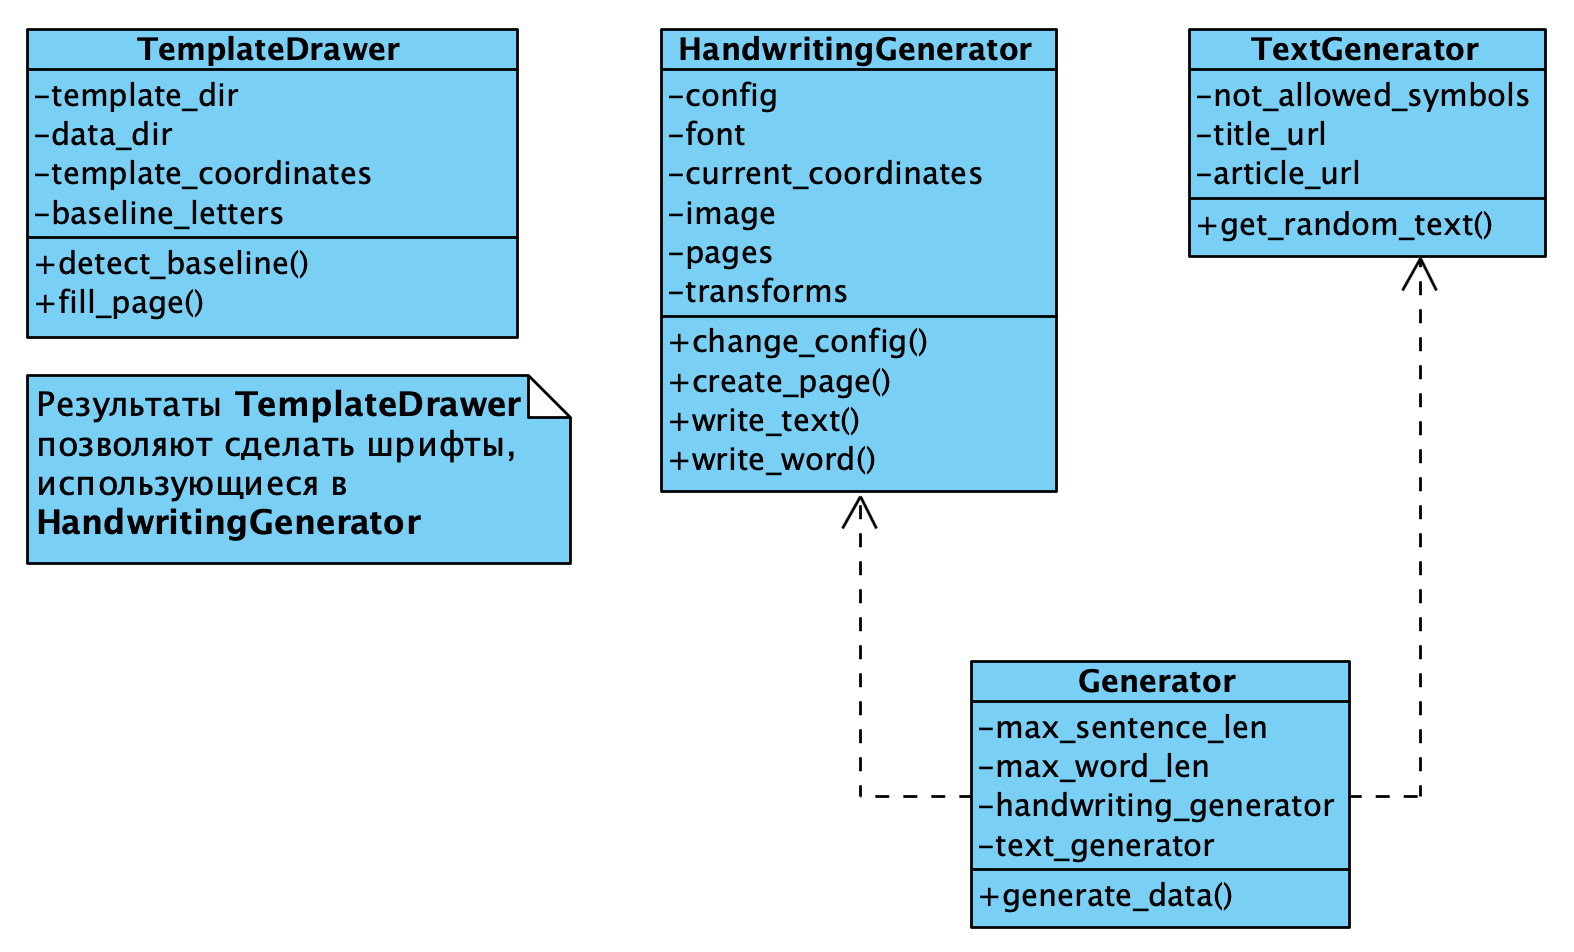
\includegraphics[width=\textwidth]{img/diagram_handwriting_generation}
    \caption{Диаграмма классов модуля генерации изображений рукописного текста}
    \label{fig:diagram_handwriting_generation}
\end{figure}

Показанные на рисунке~\ref{fig:diagram_handwriting_generation} классы позволяют осуществлять следующее:
\begin{itemize}
    \item \textit{TemplateDrawer} -- заполнение шаблона для приложения \textit{calligraphr}\footnote{\url{https://www.calligraphr.com}} для создания рукописных шрифтов;
    \item \textit{HandwritingGenerator} -- создание изображений рукописного текста с возможностью рандомизации стиля написания и фона;
    \item \textit{TextGenerator} -- генерация случайных текстов методом скачивания статей из Википедии\footnote{\url{https://ru.wikipedia.org}} и их очистки от неподдерживаемых символов;
    \item \textit{Generator} -- непосредственно генерация синтетического набора данных, включая генерацию текстов с их последующей отрисовкой.
\end{itemize}

Полученная реализация позволяет отрисовывать набор символов русского алфавита вместе с цифрами в среднем за 0.6 секунды
на компьютере MacBook Pro с процессором 1.4GHz Quad-Core Intel Core i5 и памятью 8GB 2133MHz LPDDR3.
Временная оценка работы генератора текста варьируется в зависимости от скорости работы сети, а также от длины статей, получаемых случайным образом.


\subsection{Реализация экспериментальной части}
\label{subsec:hrtr}

Реализация экспериментов, результаты которых описаны в секции~\ref{subsubsec:experiments_results}, находится в репозитории \url{https://github.com/NastyBoget/hrtr}.
В него включен отредактированный код моделей AttentionHTR и трансформера, а также их обучения и оценки качества распознавания.
Кроме того, важной частью является предварительная работа с данными -- их загрузка и приведение к унифицированному виду.
Для этого в репозитории есть специальный модуль, описанный в секции~\ref{subsubsec:datasets-processing}.
Далее более подробно описана реализация экспериментальной части.

\subsubsection{Создание и публикация дополнительных обучающих наборов данных}
\label{subsubsec:datasets-processing}

Прежде чем приступить к обучению моделей распознавания, необходимо иметь обучающий набор данных, представленный с специальном виде.
Для этого на языке \textit{Python} реализован модуль \textit{process\_datasets}, в котором каждый набор данных обрабатывается отдельным классом.
Диаграмма реализованных классов представлена на рисунке~\ref{fig:diagram_process_datasets}.

\begin{figure}[h!]
    \centering
    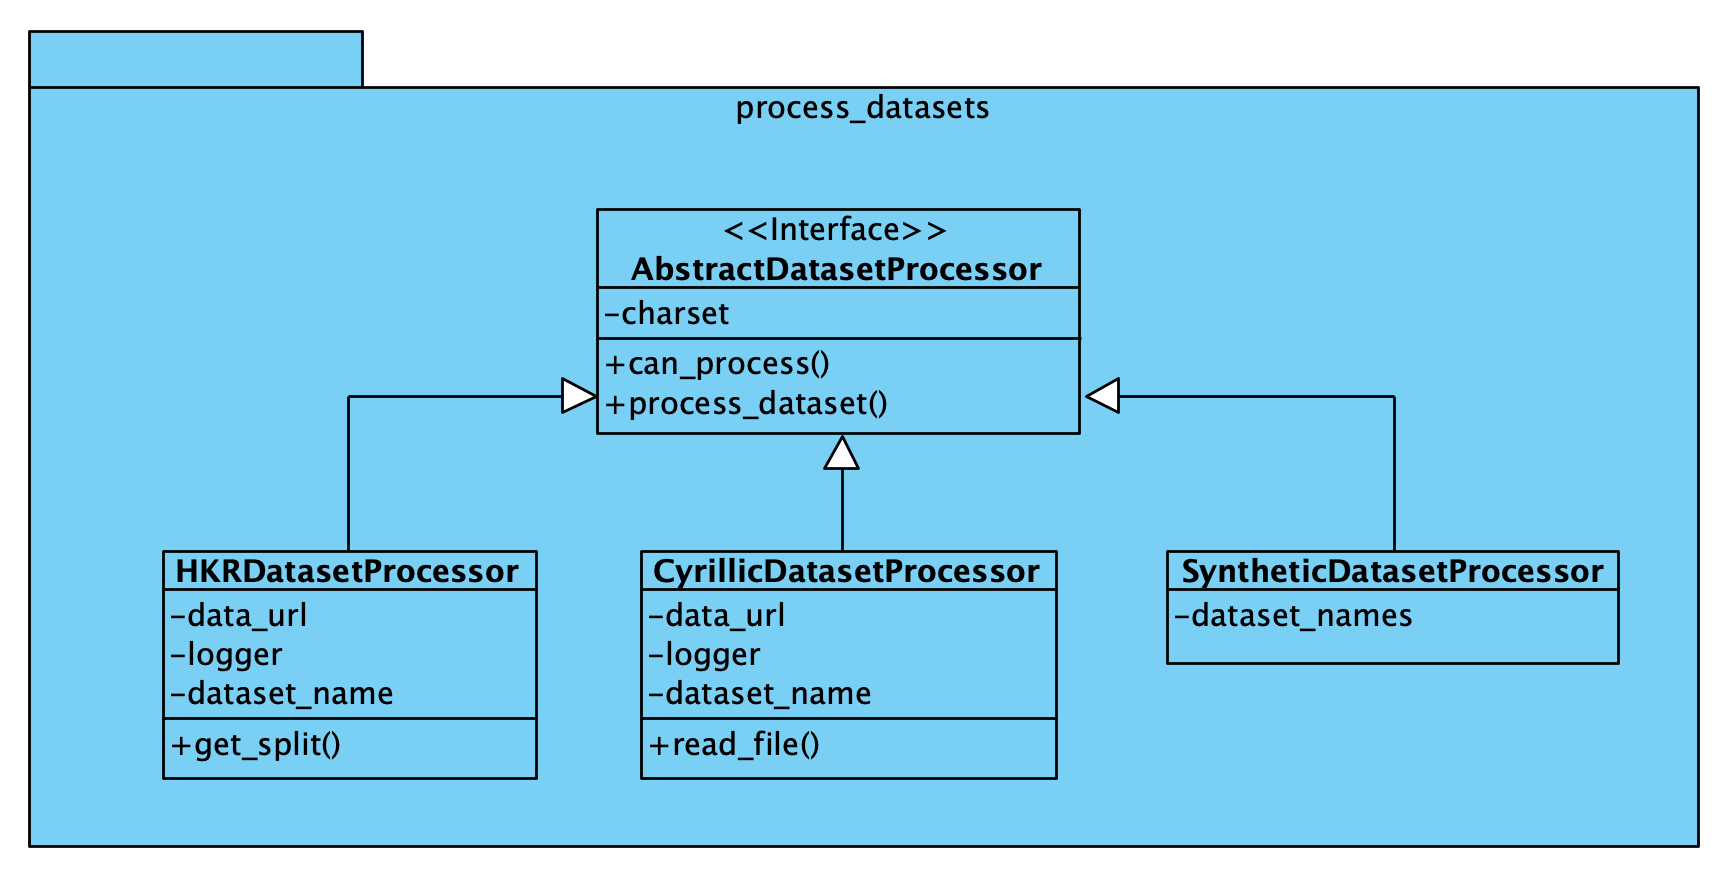
\includegraphics[width=\textwidth]{img/diagram_process_datasets}
    \caption{Диаграмма классов модуля загрузки и обработки наборов данных}
    \label{fig:diagram_process_datasets}
\end{figure}

Классы \textit{HKRDatasetProcessor} и \textit{CyrillicDatasetProcessor} используются для загрузки и обработки наборов данных HKR и Cyrillic Handwriting Dataset соответственно.
Класс \textit{SyntheticDatasetProcessor}, изображенный на рисунке~\ref{fig:diagram_process_datasets}, отвечает за обработку дополнительных наборов данных, сгенерированных автоматически.
В нём происходит загрузка наборов данных с \url{https://huggingface.co}, процесс генерации которых описан в главе~\ref{sec:Chapter3}, а именно:
\begin{itemize}
    \item Дополнение набора HKR сгенерированными данными с помощью шрифтов\footnote{\url{https://huggingface.co/datasets/nastyboget/synthetic_hkr}};
    \item Дополнение набора HKR сгенерированными данными с помощью Stackmix\footnote{\url{https://huggingface.co/datasets/nastyboget/stackmix_hkr}};
    \item Дополнение набора HKR сгенерированными данными с помощью ScrabbleGAN\footnote{\url{https://huggingface.co/datasets/nastyboget/gan_hkr}};
    \item Дополнение набора Cyrillic Handwriting Dataset сгенерированными данными с помощью шрифтов\footnote{\url{https://huggingface.co/datasets/nastyboget/synthetic_cyrillic}};
    \item Дополнение набора Cyrillic Handwriting Dataset сгенерированными данными с помощью Stackmix\footnote{\url{https://huggingface.co/datasets/nastyboget/stackmix_cyrillic}};
    \item Дополнение набора Cyrillic Handwriting Dataset сгенерированными данными с помощью ScrabbleGAN\footnote{\url{https://huggingface.co/datasets/nastyboget/gan_cyrillic}};
\end{itemize}

Для удобной загрузки и распаковки синтетических данных \textit{huggingface.co} предлагает API, которое позволяет с помощью
скрипта на языке \textit{Python} задать принцип, по которому формируется загружаемый набор данных.
На основе этого скрипта библиотека \textit{datasets} позволяет загружать и приводить данные к заданному виду при помощи одной строки кода.
Таким образом, для каждого из наборов был написан соответствующий скрипт, а класс \textit{SyntheticDatasetProcessor}
завершает более специфическую обработку данных в контексте других наборов.


\subsubsection{Обучение и оценка качества моделей распознавания}
\label{subsubsec:models-train-evaluation}

При наличии загруженных наборов данных можно приступать к обучению и оценке качества моделей распознавания рукописного текста.
Описание реализации архитектур двух моделей распознавания рукописного текста, их обучения и оценки качества представлено на рисунке~\ref{fig:diagram_hrtr}.

\begin{figure}[h!]
    \centering
    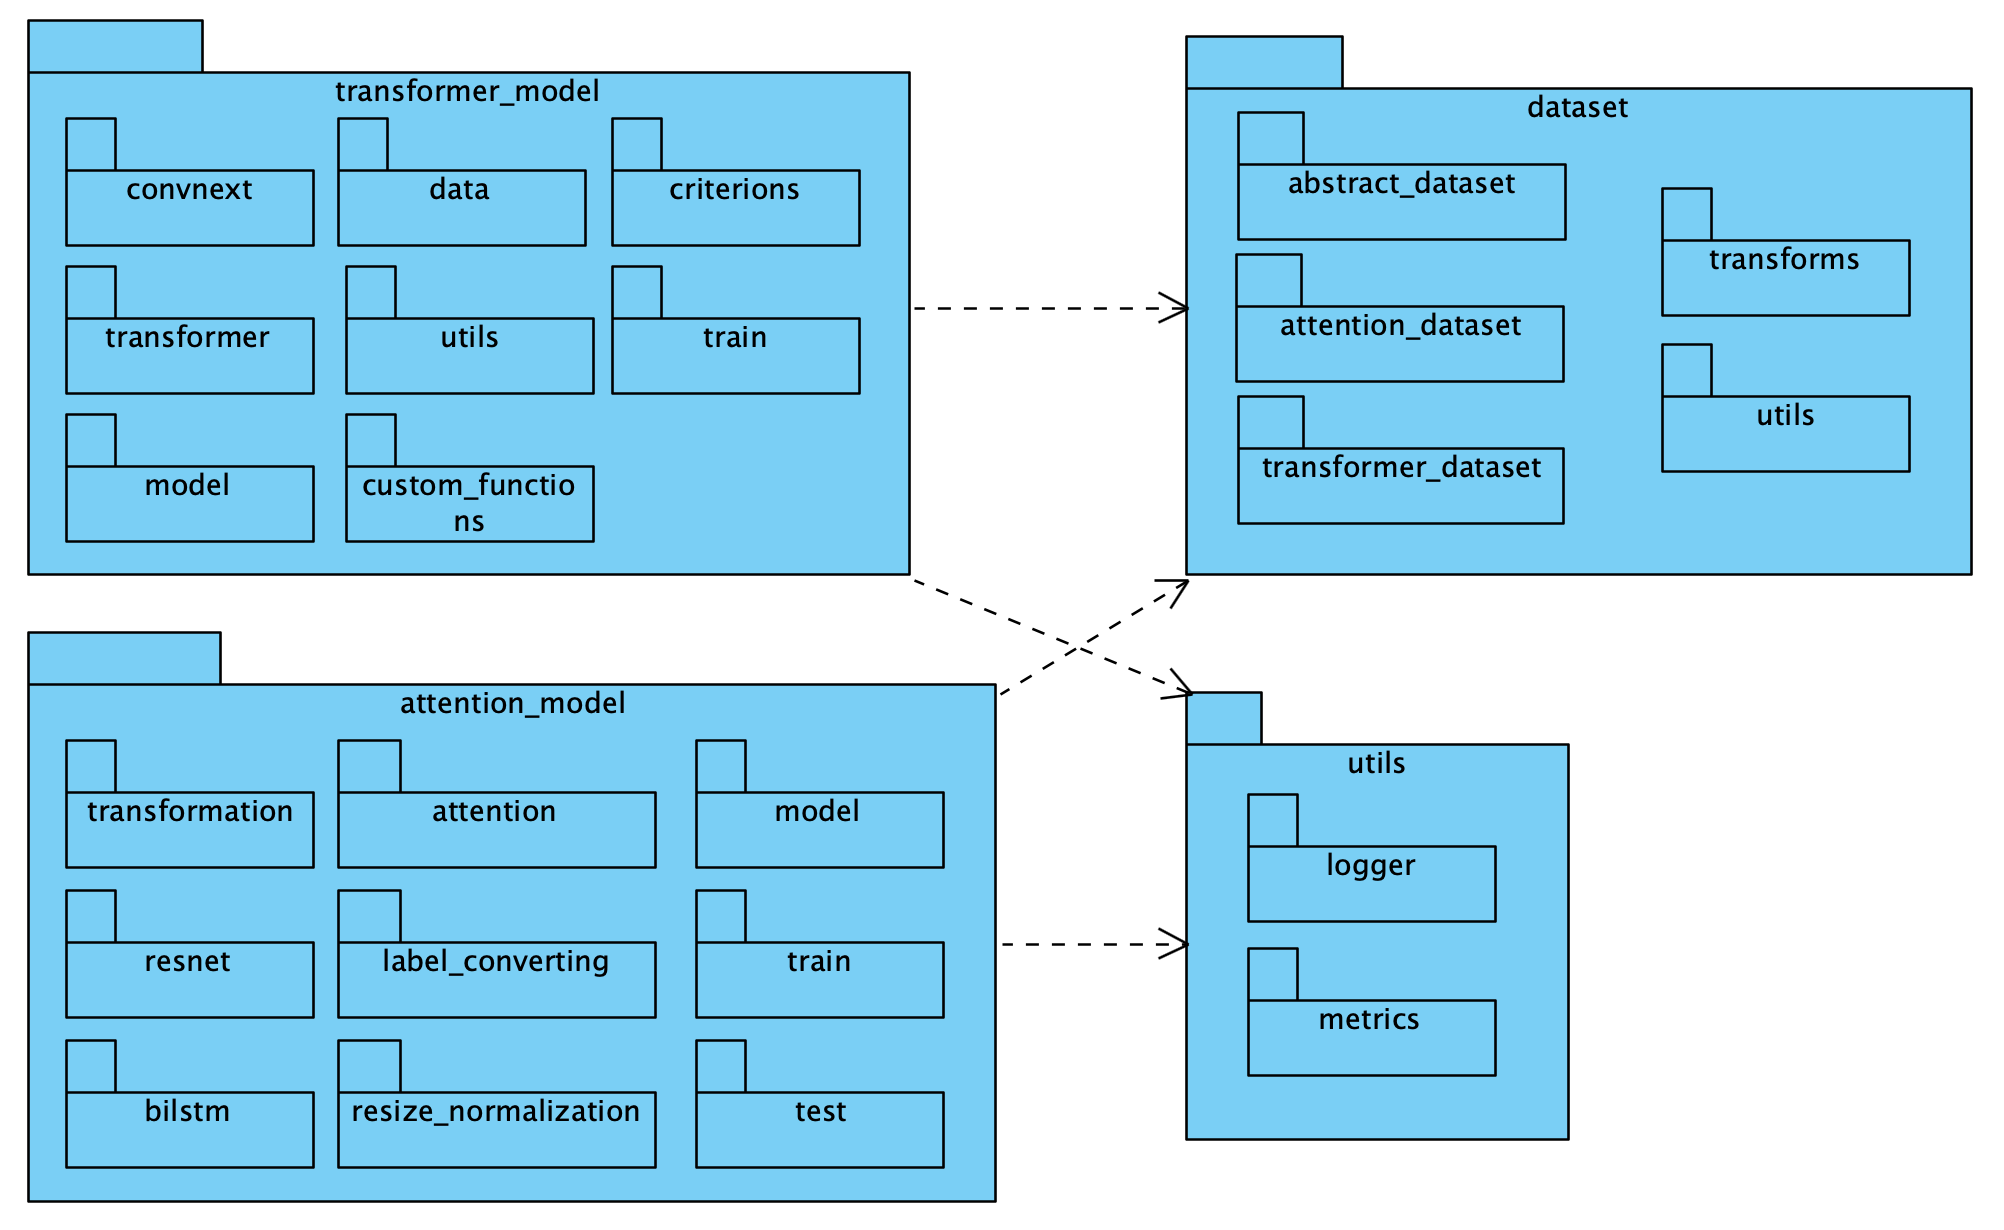
\includegraphics[width=\textwidth]{img/diagram_hrtr}
    \caption{Диаграмма пакетов для реализации обучения моделей и оценки качества}
    \label{fig:diagram_hrtr}
\end{figure}

Рисунок~\ref{fig:diagram_hrtr} описывает следующую структуру исходного кода:
\begin{itemize}
    \item Пакет \textit{utils} содержит вспомогательный код для логгирования процесса создания наборов данных и обучения,
    а также реализацию метрик оценки качества.
    Данный код написан самостоятельно для облегчения проведения всех необходимых экспериментов.
    \item Пакет \textit{datasets} содержит переопределение класса \textit{Dataset} библиотеки \textit{torch},
    сделанное для осуществления равномерной выборки данных их разных наборов в процессе обучения.
    Данный пакет содержит адаптеры, позволяющие специфичным образом обрабатывать данные для выбранных моделей распознавания.
    Помимо этого, в пакете находится фиксированный набор аугментаций, использующийся при обучении моделей,
    а также вспомогательная функция определения символьного набора данных.
    Данный пакет также реализован самостоятельно.
    \item Пакет \textit{attention\_model} содержит модифицированный код модели AttentionHTR\footnote{\url{https://github.com/dmitrijsk/AttentionHTR}}
    распознавания текста на английском языке.
    Составляющие пакета описывают архитектуру модели: модуль трансформации, модуль извлечения признаков resnet,
    модуль разметки последовательности bilstm, а также модуль декодирования attention.
    Модуль model позволяет собрать все предыдущие воедино, label\_converter используется для преобразования символов в численное представление и обратно,
    resize\_normalization используется для предобработки изображений перед их подачей на вход сети.
    Модули train и test используются для обучения модели и оценки результатов ее обучения соответственно.
    \item Пакет \textit{transformer\_model} содержит модифицированный код модели трансформер\footnote{\url{https://github.com/t0efL/end2end-HKR-research}}
    распознавания текста на английском и русском языках.
    Составляющие пакета convnext, transformer и model содержат реализацию архитектуры модели, data позволяет кодировать и декодировать символьные метки для изображений,
    custom\_functions, criterions и utils используются в процессе обучения модели, который реализован в модуле train.
    Там же находится код для оценки качества обученной модели.
\end{itemize}

Таким образом, реализованы все необходимые инструменты, использующиеся для проведения экспериментов и получения численных результатов
для сравнения методов генерации дополнительных обучающих наборов данных.

\subsection{Выводы}
\label{subsec:prac_conclusions}

В результате проделанной работы был реализован генератор изображений рукописного текста для русского языка на основе шрифтов\footnote{\url{https://github.com/NastyBoget/HandwritingGeneration}}.
Этот способ наряду с существующими реализованными методами был использован для получения дополнительных обучающих данных,
сформированные синтетические наборы находятся в открытом доступе на сайте \url{https://huggingface.co}.
Для проведения экспериментов реализованы модули обработки и унификации наборов данных, а также скрипты обучения и
оценки качества моделей распознавания рукописного текста.
Исходный код всех экспериментов находится в публичном доступе\footnote{\url{https://github.com/NastyBoget/hrtr}},
что позволяет воспроизвести полученные в работе результаты. % Описание Экспериментальной части
\section{Заключение}
\label{sec:Chapter5} \index{Chapter5}
\todo[inline]{Здесь надо перечислить все результаты, полученные в ходе работы. Из текста должно быть понятно, в какой мере решена поставленная задача.} % Заключение

\nocite{*}
\bibliographystyle{gost71u} % Для соответствия требованиям об оформлении списка литературы
\bibliography{references}


\end{document}
